\documentclass[10pt]{beamer}
\usetheme{Malmoe}
\setbeamertemplate{navigation symbols}{}
%\colorlet{beamer@blendedblue}{blue!40!black}
\setbeamertemplate{navigation symbols}{}
\newcommand*\oldmacro{}%
\let\oldmacro\insertshorttitle%
\renewcommand*\insertshorttitle{%
\oldmacro\hfill%
\insertframenumber\,/\,\inserttotalframenumber}

\usepackage{caption}
\usepackage{hyperref}
\usepackage[makeroom]{cancel}
\usepackage{ amssymb }
\usepackage{appendixnumberbeamer}
%\usepackage{tikz-feynman}
\usepackage{graphicx}
\begin{document}

\title{Nationwide: Model Risk Management Assessment/Case Study}
\author[Barkeloo]{Jason Barkeloo, Ph.D.}
\date{November 16, 2020}

%\titlegraphic{\includegraphics[width=4cm]{../ATLAS-Logo-Ref-RGB.png}\hspace*{2.75cm}~%
%   \includegraphics[width=4cm]{../uo_logo_green_on_white_2.jpg}
%}

\frame{\titlepage}
\frame{\frametitle{Table of Contents}\tableofcontents[hidesubsections]}

\frame{\frametitle{Code location for further fleshed out examples}

All code for these exercises can be found via this hyperlink as ipython/jupyter notebooks located on my github in addition to attachments sent with the presentation: \\~\\


\hyperlink{https://github.com/JTBarkeloo/JupyterNotebooks/blob/master/MRM Assessment.ipynb}{https://github.com/JTBarkeloo/JupyterNotebooks/blob/master/MRM Assessment.ipynb} 

}

\section{Exploratory Analysis}

\frame{\frametitle{Exploratory Data Analysis}
\begin{itemize}
\item Start by looking at behavior of noncategorical data
\end{itemize}
\centering
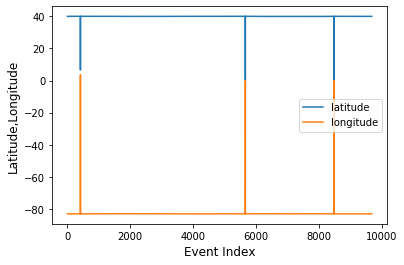
\includegraphics[width=0.45\textwidth]{Images/Image1.png}
\begin{columns}
\begin{column}{0.5\textwidth}

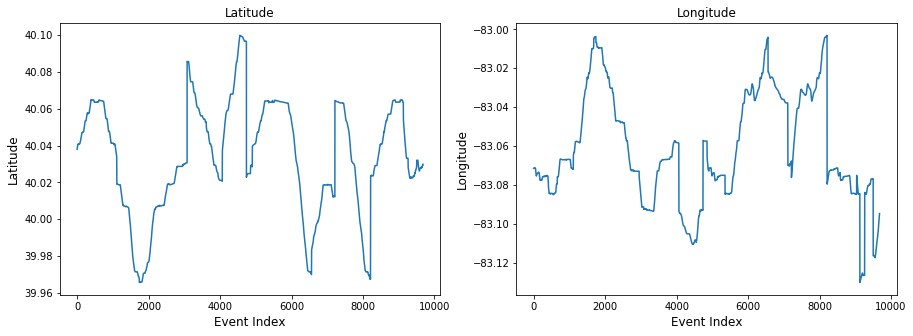
\includegraphics[width=0.9\textwidth]{Images/Image2.png}
\end{column}
\begin{column}{0.5\textwidth}
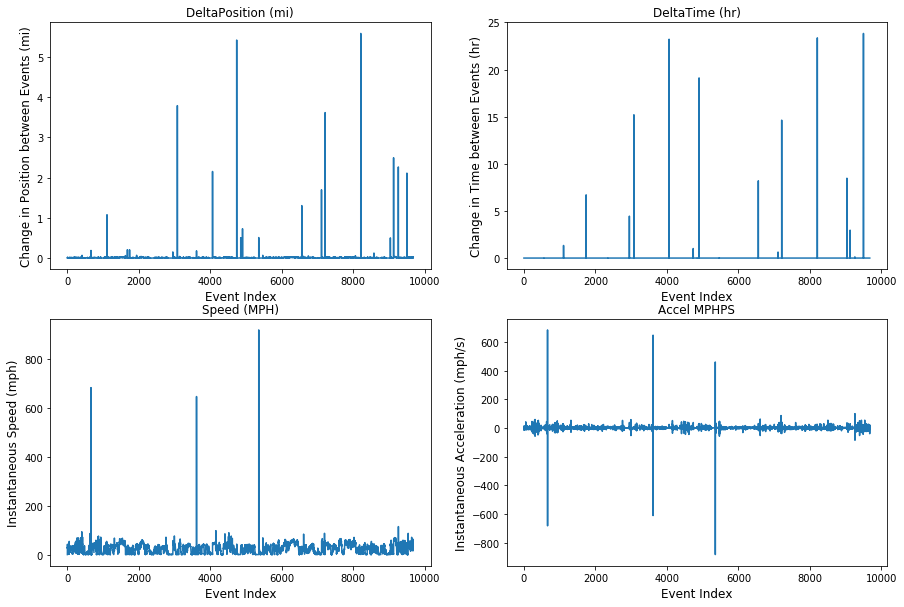
\includegraphics[width=0.9\textwidth]{Images/Image3.png}
\end{column}
\end{columns}
}

%\frame{\frametitle{Further Cleaning - $\Delta$Position, $\Delta$Time, Speed, Acceleration}
%\centering
%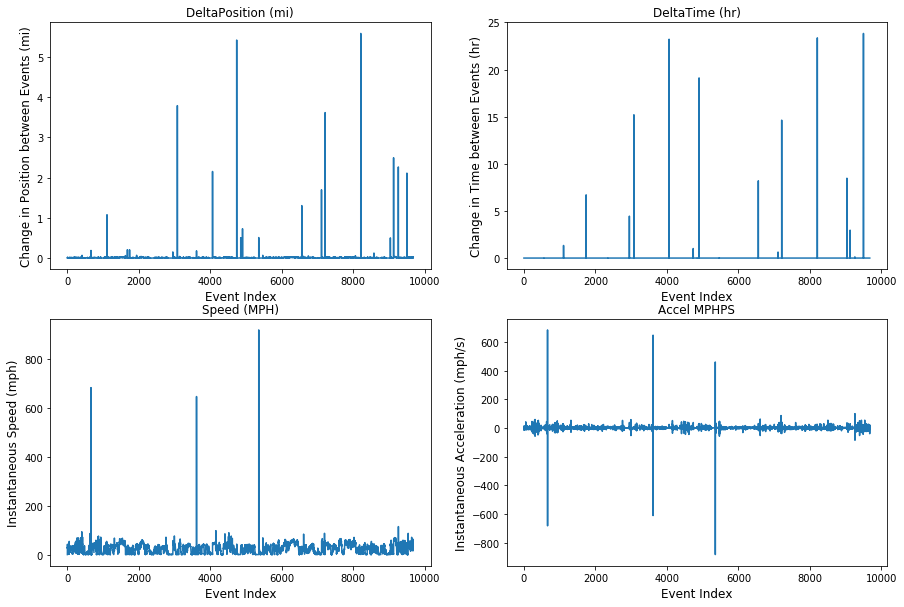
\includegraphics[width=1.\textwidth]{Images/Image3.png}
%}



%%%%%%%%%%%%%%%%%%%%%%%%%%%%%%%%%%%%%%%%%%%%%%%%%%%%%%%%%%%%%%%%%
\section{Model Building}
\frame{\frametitle{Model Building}
Summary of 30,000 vehicles 1Hz telematics datasets
\begin{itemize}
\item Vehicle - Effectively an index on the data
\item Days - Number of days data was collected (365 for all)
\item Distance - Total number of miles vehicle was driven during data collection
\item HardBrakes - Number of hard braking events detected
\item HardAccelerations - Number of hard acceleration events detected
\item NightTime\_Pct - Percentage of total miles driven at night
\item VehicleType - str description of type of vehicle
\item Loss - Indicator if vehicle has been in a collision
\end{itemize}
Want to build a model that will optimize recognition of Loss events using these values
%\centering
%\includegraphics[width=0.7\textwidth]{../../ThesisImages/backgrounds.png}
}

\frame{\frametitle{Statistical Significance Between Vehicle Types}
The conclusions to be drawn depend on how liberal the definition of statistical significance being used is \\ 
The use of p$<$0.05 is somewhat arbitrary but is what will be used here as it is a standard choice of convention
\begin{itemize}
\item \fbox{z value for Car and Minivan: 2.48} 
\item z value for Car and SUV: 4.19 
\item z value for Car and Truck: 2.96 
\item z value for Minivan and SUV: 4.59 
\item z value for Minivan and Truck: 3.92 
\item \fbox{z value for SUV and Truck: 1.62} 
\end{itemize}
The null hypothesis cannot be rejected for the combination of Cars and Minivans and the combination of SUVs and Trucks \\
The implication then is that there are 2 distributions being sampled for these simulated events. This matches intuition as Trucks/SUVs exist in a cargo-loading domain while Cars/Minivans are what parents may gravitate toward% which would describe the necessity of multiple distributions
}




%%%%%%%%%%%%%%%%%%%%%%%%%%%%%%%%%%%%%%%%%%%%%%%%%%%%%%%%%%%%%%%%%%
\subsection{Model Building}

\frame{\frametitle{Model Building}
Primarily employing densely connected feed forward neural networks for event classification was chosen as it is the machine learning model I have most experience with for binary classification
\begin{itemize}
\item 1 input layer with all potentially useful features (Distance, HardBrakes, HardAccelerations, NightTime\_Pct, VehicleType)
\item blah
\end{itemize}
A training (64\%)/testing(16\%)/validation(16\%) random set split was done to help ensure unbiased results
%\centering
%\includegraphics[width=0.7\textwidth]{../../ThesisImages/backgrounds.png}
}

\frame{\frametitle{Naive Approach Neural Network}
\begin{itemize}
\item Naively we could train a neural network on the data classes as given
\item With enough separation power i.e., variables distinct enough in each class, this can be used for event classification
\item This is not the case for this dataset, only a few variables inputs with a lot of distribution overlap
\item This would then be expected to fail with a total accuracy that trends toward the class representation of the majority class, which is seen here
\end{itemize}
\begin{columns}
\begin{column}{0.5\textwidth}
\includegraphics[width=0.9\textwidth]{Images/Image11.png}
\end{column}
\begin{column}{0.5\textwidth}
%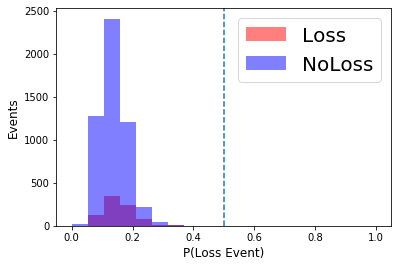
\includegraphics[width=0.9\textwidth]{Images/Image12.png}
\end{column}
\end{columns}
}

\frame{\frametitle{Neural Network with SMOTE Upsampling}
\begin{itemize}
\item Another network was created and trained using Synthetic Minority Oversampling Technique (SMOTE) over-sampling with similar results
\item SMOTE generates synthetic data that is similar to, but not exactly like the minority class, using a nearest-neighbors approach and fills in space between neighbors
\end{itemize}
\begin{columns}
\begin{column}{0.5\textwidth}
%\includegraphics[width=0.9\textwidth]{Images/Image15.png}
\end{column}
\begin{column}{0.5\textwidth}
%\includegraphics[width=0.9\textwidth]{Images/Image16.png}
\end{column}
\end{columns}
Loss Events P(Loss Event): mean: 0.510, std: 0.096 \\
NoLoss Events P(LossEvent): mean: 0.480, std: 0.097 \\
Loss Event Accuracy: 55.7\%
}

\frame{\frametitle{Model Comments}
\begin{itemize}
\item  Neural networks have been created and trained on a limited set of input variable with success in determination of Loss events
\item The addition of further independent input variables would help the separation of the neural network greatly
\item A bifurcation of the distributions is starting to occur with the ADASYN network, more input variables and events is likely to cause a major splitting of the distribution into likely Loss events and likely NoLoss events \\
%\item ADASYN over-sampling focuses on the decision boundary which leads to large flucuations in the validation accuracy
\item Boosted decision tree (BDT) models were also employed in the Jupyter notebook to slightly different ends
\end{itemize}
}

%\frame{\frametitle{}
%}

\section{Model Assessment}

\subsection{Model Limitations}
\frame{\frametitle{Title}
Can Multiple Loss Models be Useful Based on Driver Class i.e., Rural Vs. Urban Drivers?
\begin{itemize}
\item Rural and Urban drivers face different landscapes of challenges on their daily travels
\item Requirement: GPS definition of urban environments
\item Expect longer distance/trip for rural drivers while urban drivers have more stop-and-go traffic 
\item Larger Distances and a larger amount of HardAccelerations are both positvely correlated with loss this seems to be an interesting intersection of these correlations
\end{itemize}
\centering
%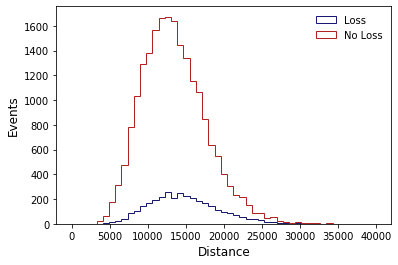
\includegraphics[width=0.4\textwidth]{Images/image18.png}
}

%\frame{\frametitle{Conclusion}
%\begin{itemize}
%\item Orthogonal validation/control regions are in development
%\end{itemize}
%}


%%%%%%%%%%%%%%%%%%%%%%%%%%%%%%%%%%%%%%%%%%%%%%%%%%%%%%%%%%%%%%%%
%%%%%%%%%%%%%%%%%%%%%%%%%%%%%%%%%%%%%%%%%%%%%%%%%%%%%%%%%%%%%%%% 	
%\appendix
%\section{Backup}
%\frame{\frametitle{Backup}
%}
\end{document}

%36.070
